\documentclass[11pt, letterpaper]{article}
\usepackage{graphicx}
\usepackage{float}
\graphicspath{{./figures/}}

\title{Howl's Moving Castle}
\author{Shreyas Kalvankar}

\begin{document}

\maketitle

\hspace{0.25 in}Ghibli brings us another masterpiece in the form of Howl's Moving Castle which, in my opinion, is widely underrated and misunderstood. Its important to observe how Studio Ghibli gets more and more intricate with all the films that it produces and it clearly shows how Miyazaki matures as a director as he makes Howl's Moving Castle and how that is reflected in him making a film about adulthood. \\
\hspace{0.25 in}Howl's Moving Castle, at first watch, seems like a fairy tale, which is what most people focus on albeit failing to notice the complexity and intertwining of different layers of the movie. As with all other Miyazaki films, there are a lot of layers to Howl's moving castle. The fairy tale layer, mythology layer, environmental layer and more. The most important being that over time as Miyazaki matures as a director, his films that were already complex, become even more complex and granular. There are entire story arcs that happen within a moment that contribute to the character development. And with every re-watch, we can spot newer and newer things owing to the scenes that are so tightly packed that Miyazaki probably just wanted people watching it again and again. For instance you can see that Sophie appears different in every scene throughout the film depending on the context or the war that is developing in the background that suddenly pounces off in the latter half of the film. One can observe how Miyazaki is reusing his own symbols from his previous films in forms of metaphors that he has already introduced in a different context. Like the umbrella from Totoro. That is how the Miyazaki theory takes root in the modern standing where symbolism is at utmost importance that Miyazaki uses to convey a message. When we watch animation, we expect to see things that are out of the ordinary and Miyazaki's unique gift is to infuse the ordinary with magical qualities. 

\begin{figure}[H]
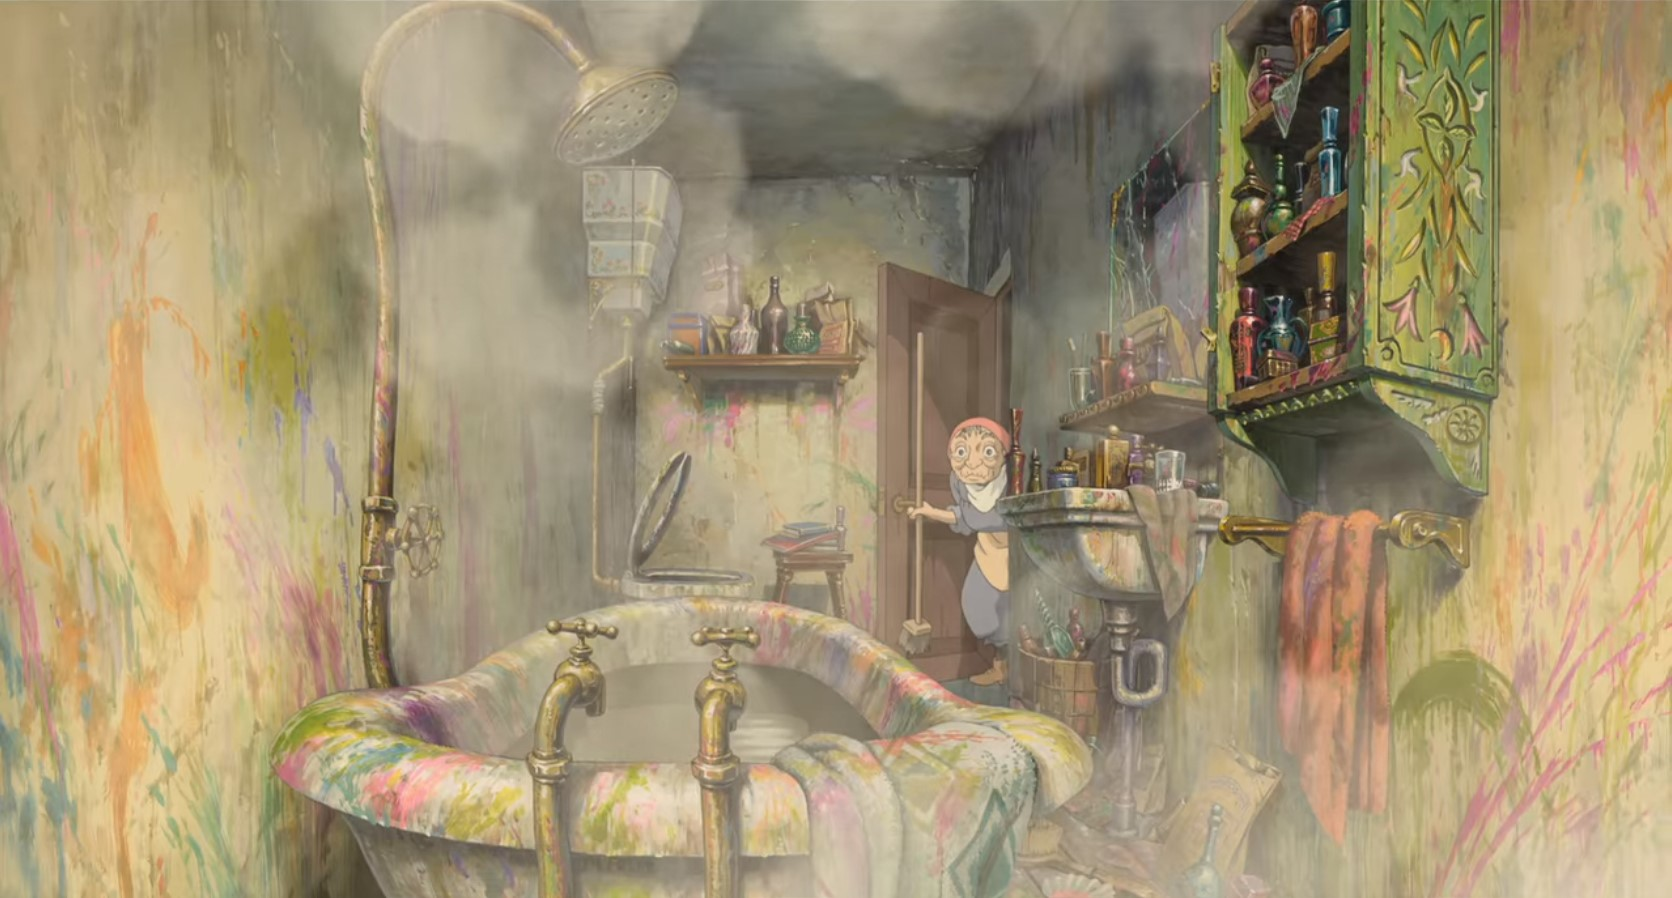
\includegraphics[width=\textwidth]{cleaning.jpg}
\centering
\end{figure}

Even the most boring of the daily chores, cleaning, is given these treatments. There is an awe inspiring attention to details and a sense of wonder in those details is what makes those scenes that much more transporting. Of course, the great thing about this film is that if you don't want, you don't have to pay attention to any of these details and go with the story because it's based so well on the characters that you can go through the story as one of them and get your own emotional breakthroughs. 

In a press conference, Miyazaki said, \textit{"While always saying that I have to or want to make films for children, in reality I often forget about them. That's how I end up creating films like Porco Rosso and Howl's Moving Castle"}. And it is interesting in the sense that this film is about adulthood more than other Miyazaki films which have some sort of \textit{coming-of-age} story going on whether its mythological or practical or growing up, trying to find solutions to the problems that your parents' generation has created or growing up by finding a place in society and the modern world. And after all these \textit{coming-of-age} stories, this is a film that stars people who are actively trying to avoid adulthood. 

Sohpie is shown to have a lovely outlook on life at the beginning of the film. She doesn't want to live her life making hats in the backroom, but her experience of life is that it's still better in there that out somewhere and that's a mutual sentiment which all introverts can empathize with. When Sophie gets her "curse", it seems quite a relief for her which is not usually how curses work. She is really quick to embrace what has happened and it means that she can skip the adulting thing entirely. 

\begin{figure}[H]
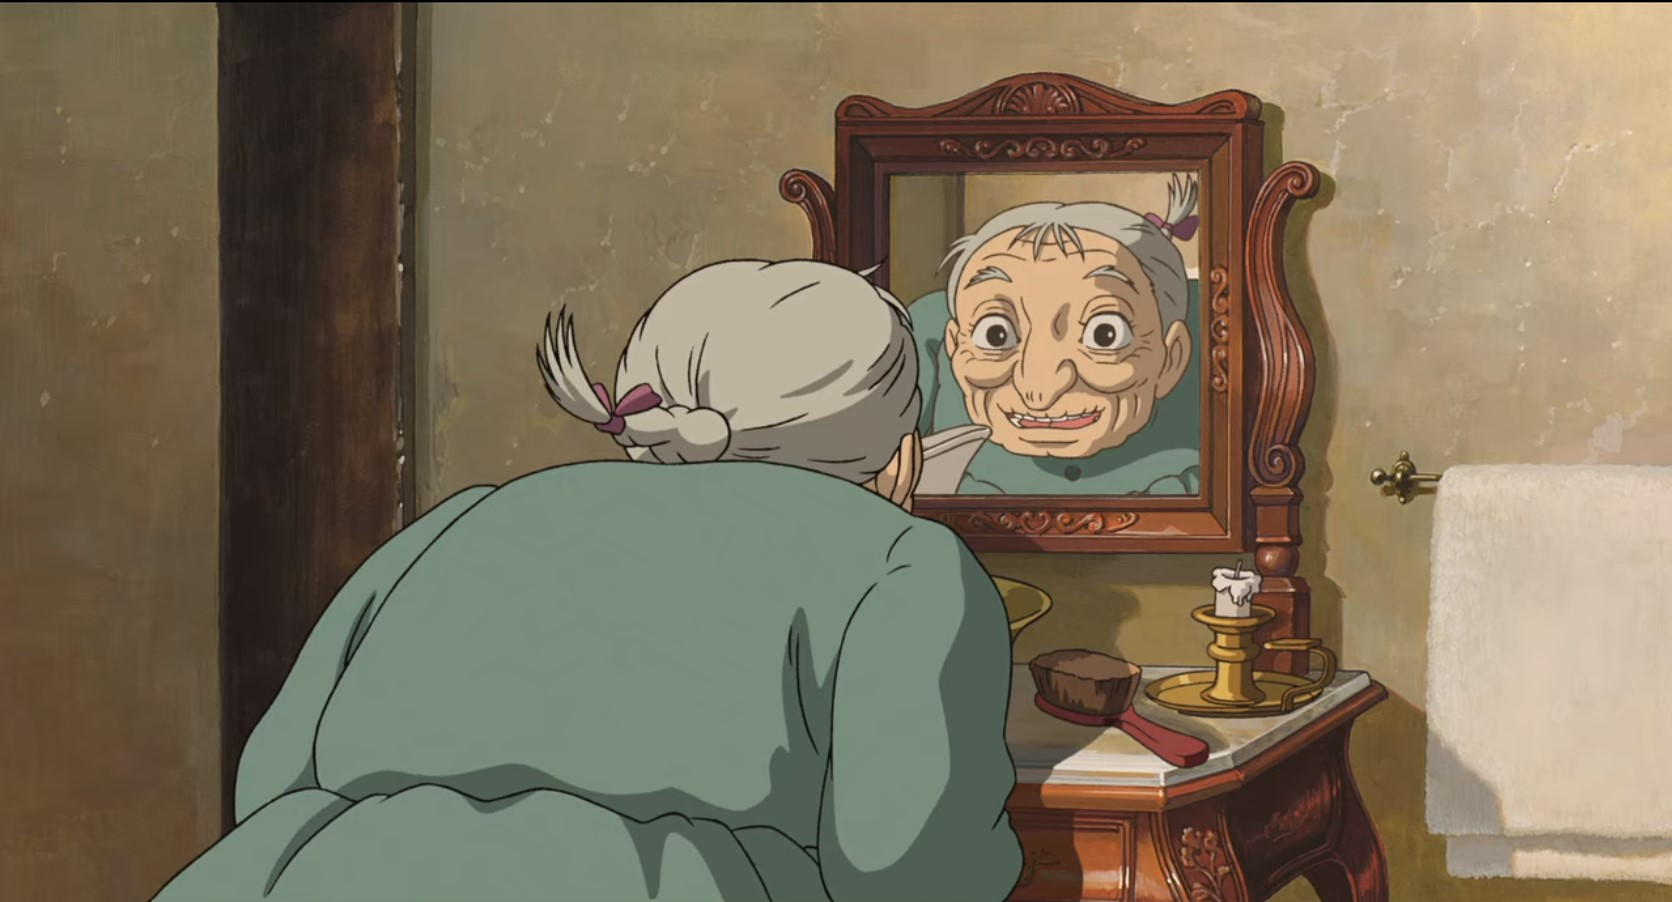
\includegraphics[width=\textwidth]{relief.jpg}
\centering
\end{figure}

Then we have Howl who is permanently stuck in adolescence. He loves the power that comes with growing up but not the responsibilities. Throughout the film he tries to be everything for everyone while being afraid of losing control of his power and not being loved. 

\begin{figure}[H]
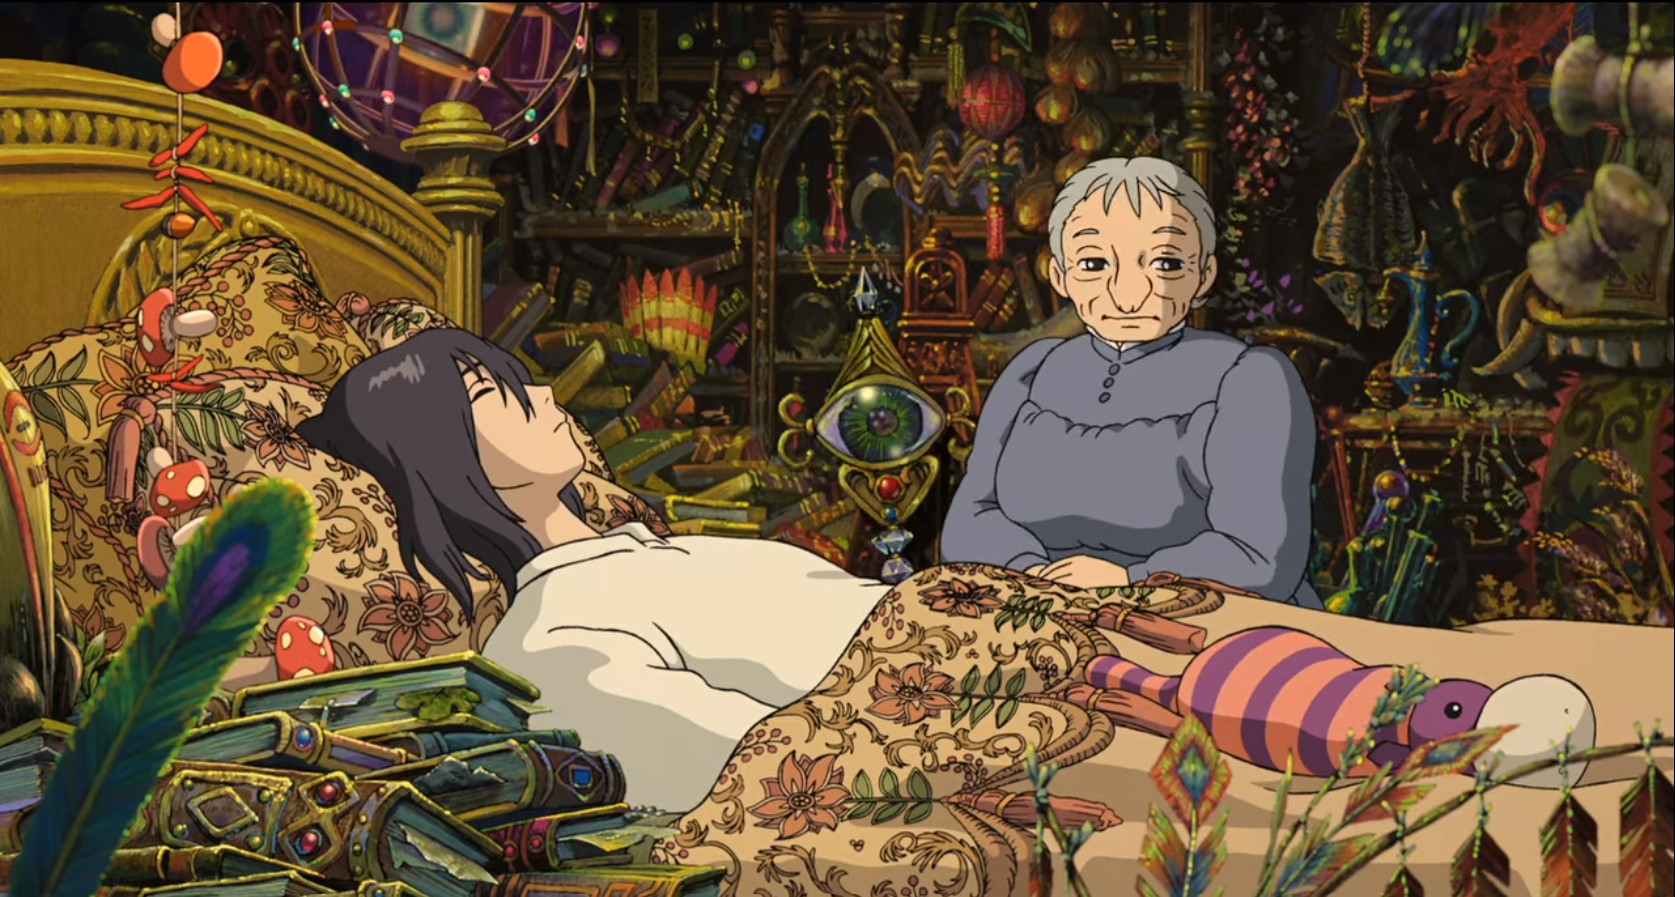
\includegraphics[width=\textwidth]{adolesence.jpg}
\centering
\end{figure} 

And his emotional breakdown reveals some of these things that his character is struggling with.

\begin{figure}[H]
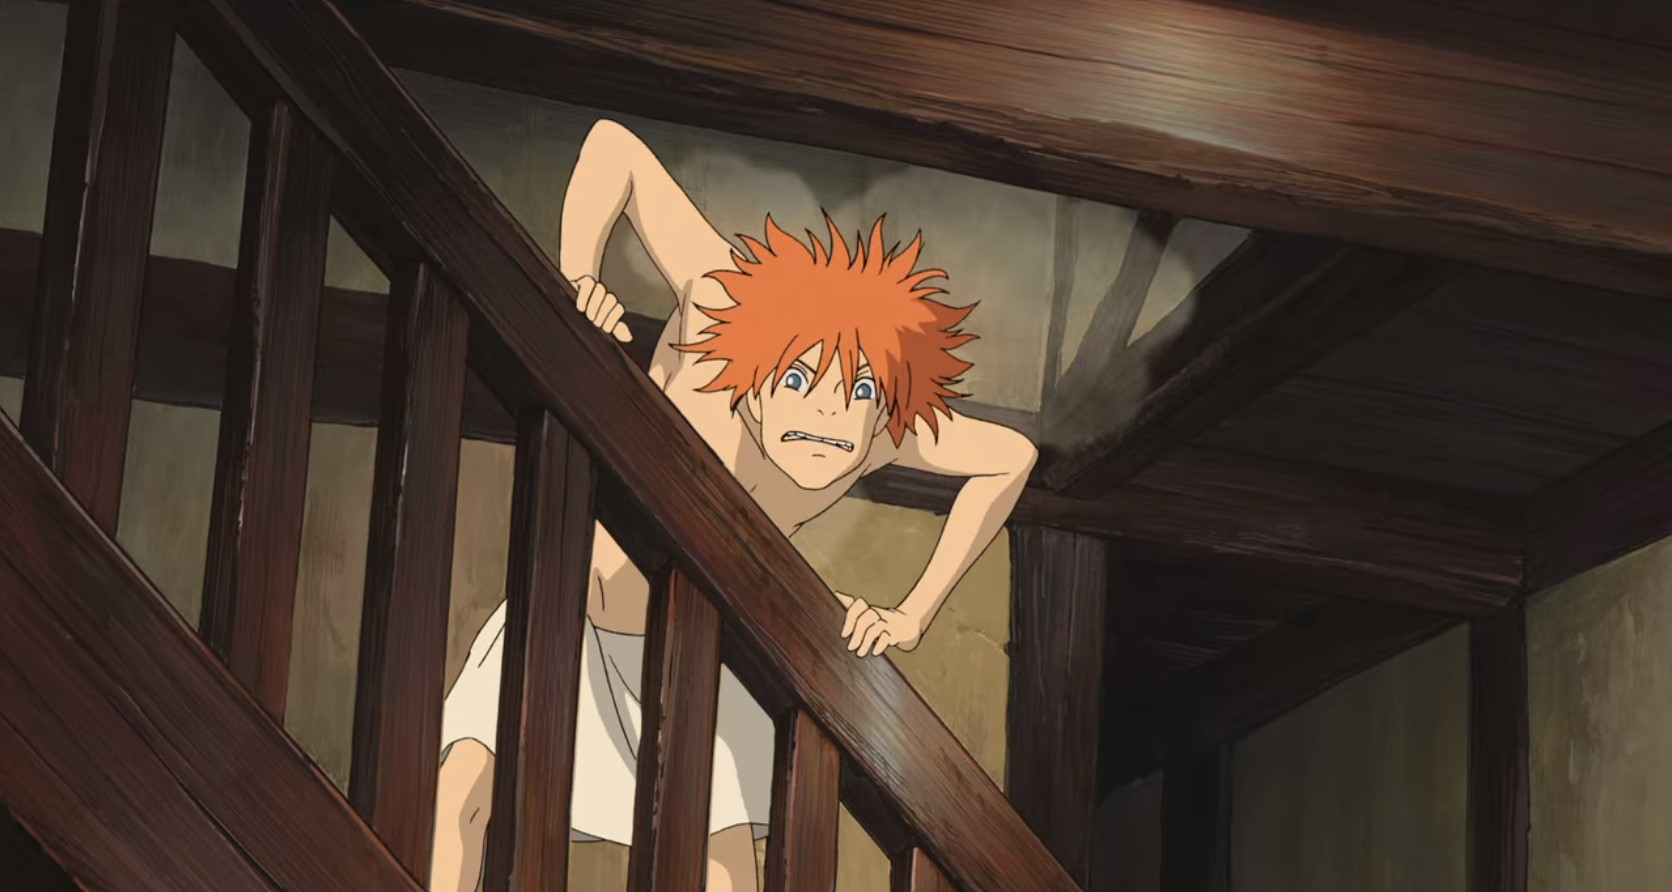
\includegraphics[width=\textwidth]{breakdown.jpg}
\centering
\end{figure}

Then there's Marco who we barely know but can deduce that he's the kind who has had to grow up too quickly for some reason. His actual job is to pretend being an adult but in the later half of the film we learned that what he needs is belonging and family. 

\begin{figure}[H]
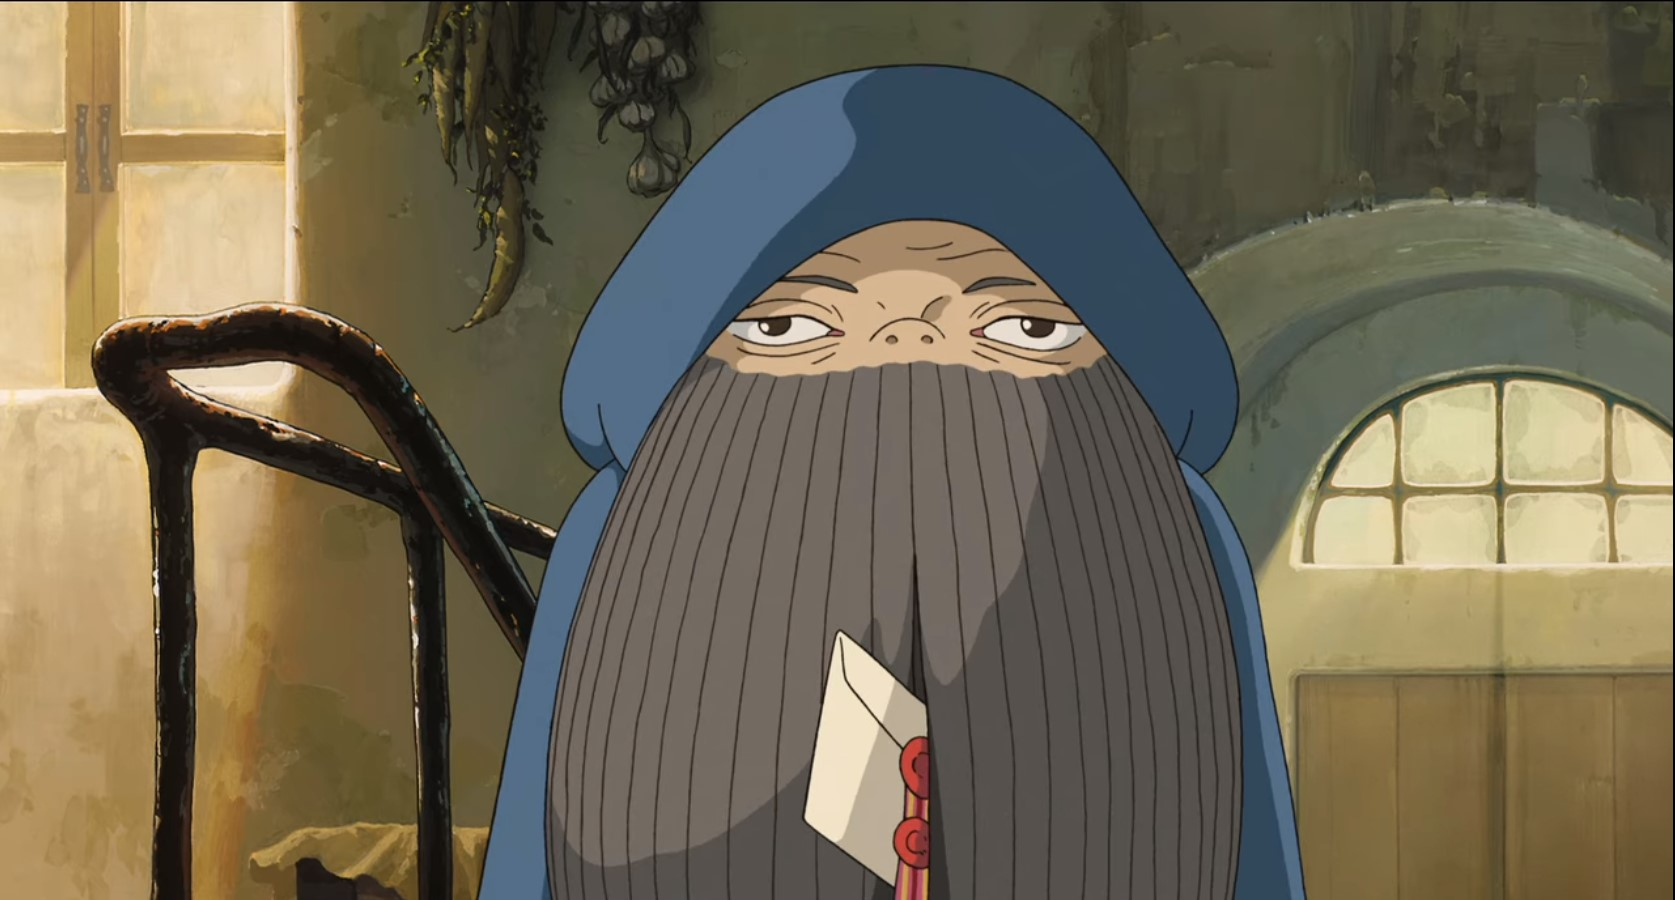
\includegraphics[width=\textwidth]{acting_old.jpg}
\centering
\end{figure}

Calcifer is the most ancient and mythological thing in the film who has ties to the Hindu God \textit{Agni}. Despite his roots, he's actually dealing with the same problems that the other characters are but in a more metaphorical sense. His question is, \textit{"What happens if I change? Can I change while remaining the same person that I am now? If I change, do I die?"}. 

\begin{figure}[H]
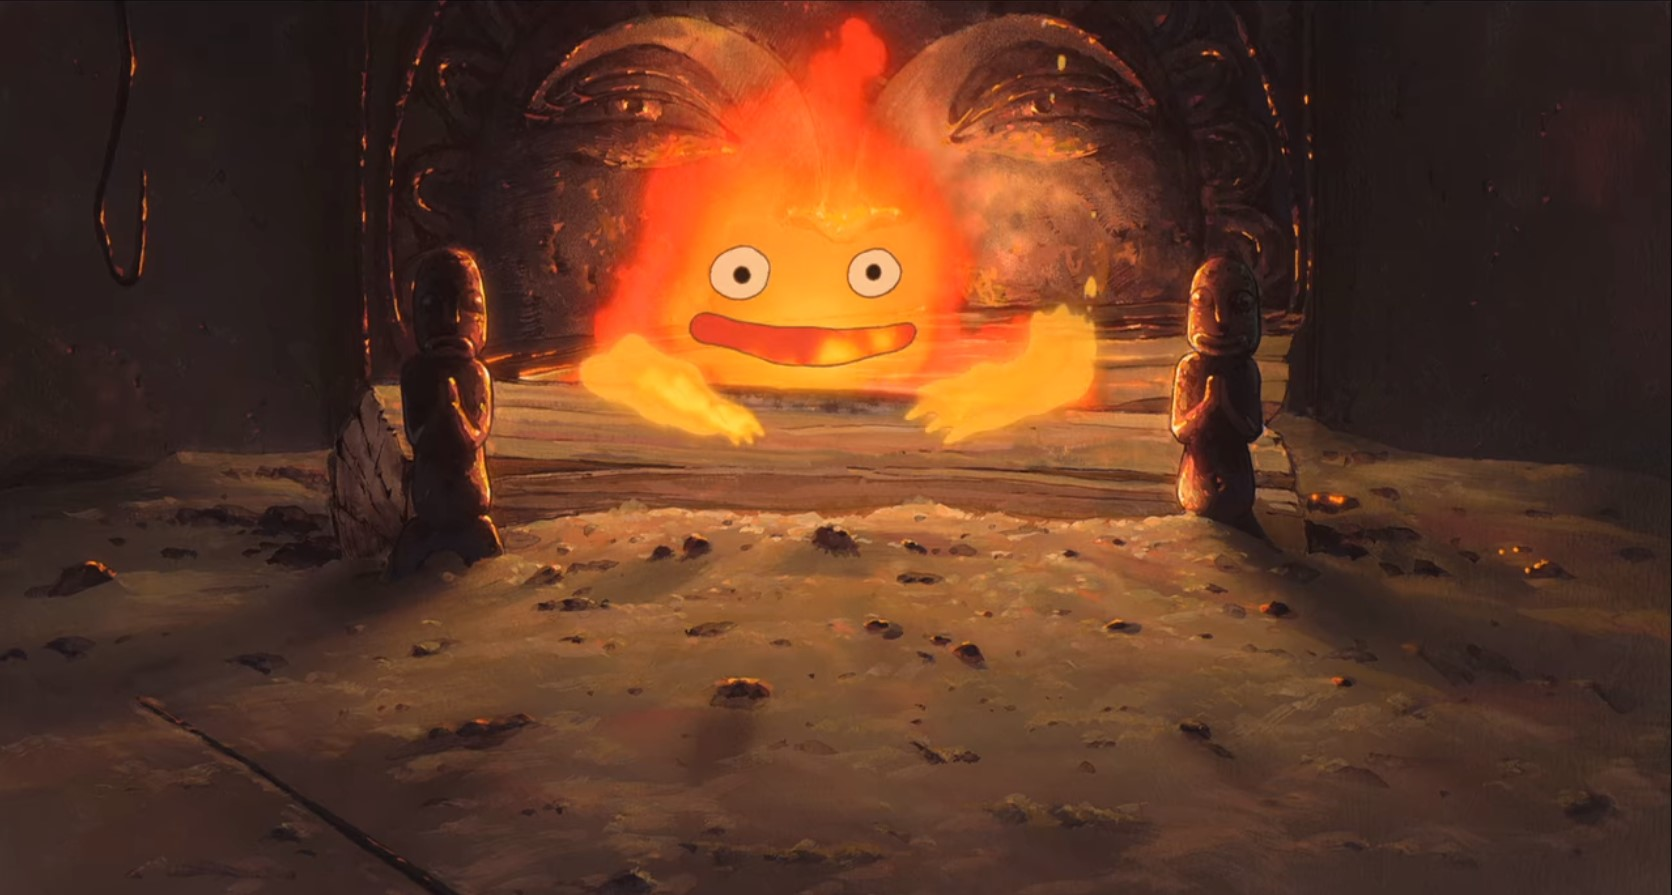
\includegraphics[width=\textwidth]{ancient.jpg}
\centering
\end{figure}

The short blink-and-you'll-miss-it story line is of the dog that has exactly one decision point in the entire film. It involves coming out of dependency and stand for something which is why he joins the adventurers. 

\begin{figure}[H]
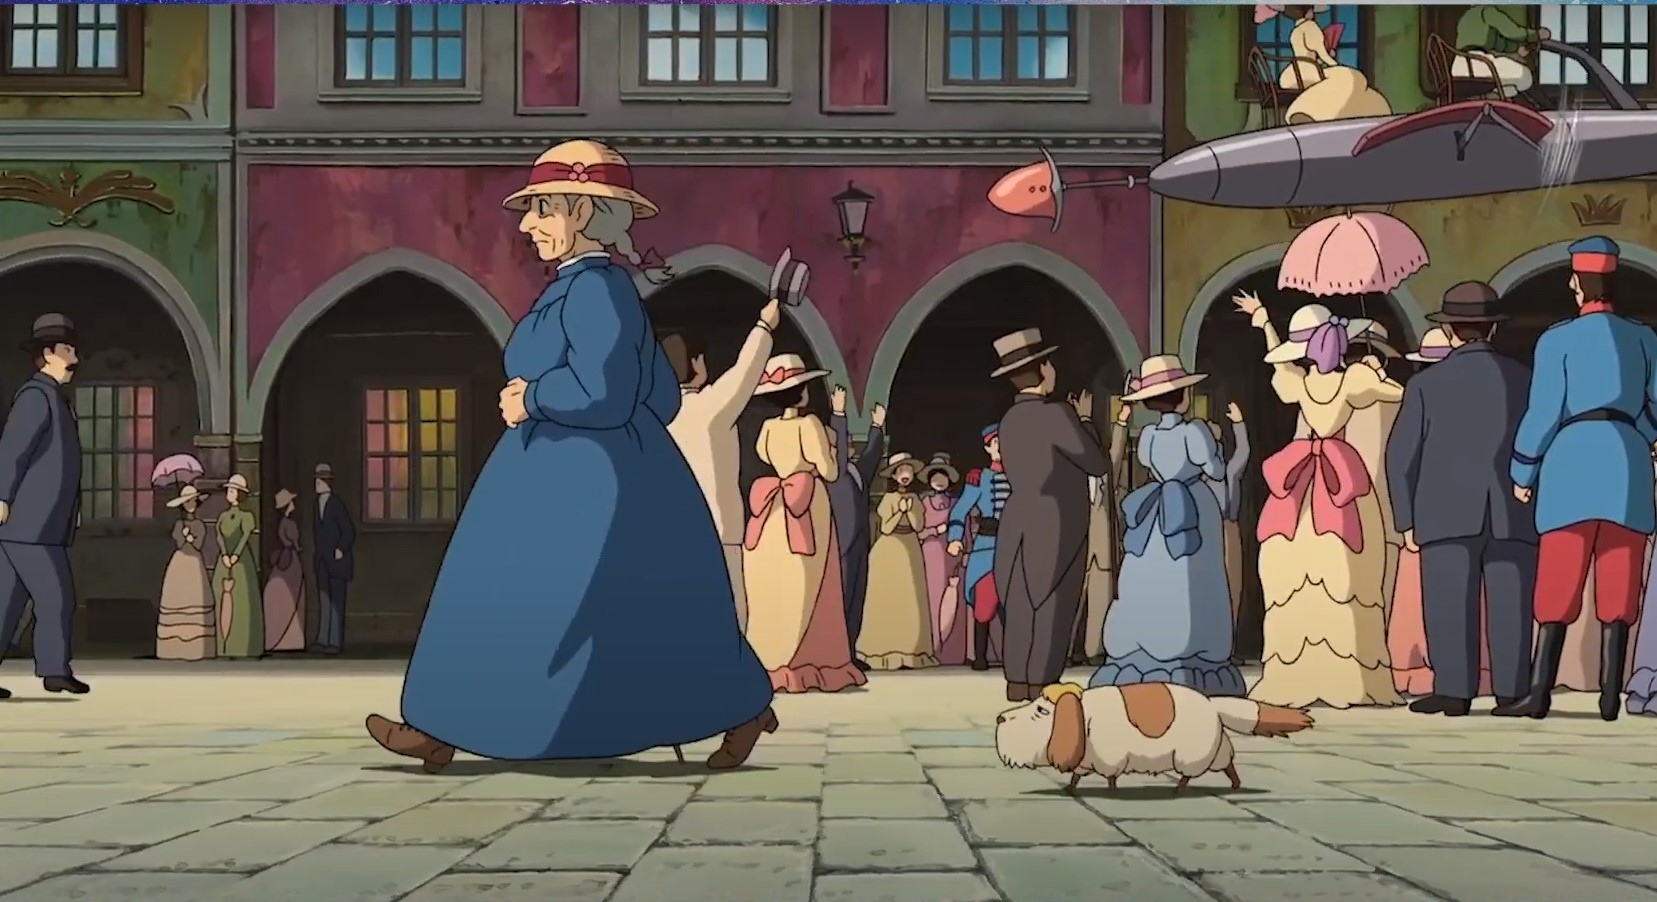
\includegraphics[width=\textwidth]{blink-and-miss.jpg}
\centering
\end{figure}

The final character is the house and people often overlook this but the house itself is a character which changes throughout the film. The question for the castle is the same as Calcifer, \textit{"What happens if I keep changing? Can I be put together again if I fall apart?"}. And this latter question poses an undertone in which the castle symbolizes Japan. And throughout the film, the castle grows and changes and it suffers but it survives all of the changes, and these were the changes needed for it to grow and become more of the house that we can all live in. 

All the characters dealing with the difference in \textit{What I show to the outside world} vs \textit{How I am really feeling?} is the Japanese separation of the outward facing facade that people put on for society's sake. Even the house has its context dependent output faces. 

The question is \textit{"Why are these people trying to avoid being adults?"}. Well, its because of what adults are like. In the film, adults are greedy, egoistic, manipulative, toxic. Looking at the adults that Sophie sees around her, her colleagues who are super shallow and gossip about having a better life but not doing anything about it. Her sister, whose life revolves around looking pretty and pleasing men in return for attention. Her mother who has a constant competition about being the best. And if that is what being an adult is like for Sophie, its no wonder that you skip it. 

Then there's Howl's adult, Soloman. A corrupt mother figure. A king who's an idiot father figure. The Witch of the waste is only interested in magic because of the greed. And all the other wizards that did what they were taught to do and ended up losing their humanity completely. 

The point that the film makes is that even though all adults are horrible, all these coping mechanisms that the characters use to avoid adulthood do not work. Escapism is not the solution. Whatever magic the characters use, the truth is under there. So they have to figure out how to become adults in a way that they stay true to themselves. Miyazaki wants the characters to live their true lives and find their true spirits. So the path that the characters realize is of finding their true selves and story of the characters is to help each other find their own true selves. The story fed is, How, who lives in the delusion that he can solve everything with careful maneuvering. And of other Miyazaki male heros, his learning curve is much steeper. Miyazaki's bottom line is that no war is worth going into. You cannot solve war by winning it. 

The ending is one of the weirder Miyazaki endings because by the end, everything resolves suddenly. But if you watch the film close enough and see the internal logic, the entire story was a set up to that ending. Miyazaki achieves this with a combination of fairy tale rules and therapy rules. In fairy tales, you find the point of the main plot and you solve it and the kingdom gets magically restored. In therapy, you get down to the core of your problem, crack it, get your breakthrough moment and the bigger the change is, the bigger is the ripple effect on your life. And that is what happens at the end of the film. People find their true hearts, literally. What is misplaced is replaced (the scarecrow), literally. And the violence stops because the need for the thing that was substituted for violence was fulfilled and there's no more need for violence. 

But the real statement is how the choice is not between becoming a horrible adult or not growing up at all. The resolution comes from the characters when they learn to define for themselves what adulthood is, what family is, what is worth making a stand for and what is making effort for and that's the kind of adult that Miyazaki would like you to be. 

\end{document}
